\subsection{Benchmarking}

The primary goal of this section is to determine a reference point for \ac{HPC} performance benchmarking, in order to establish a framework with which we can gather performance metrics using standardized tools. This framework will be applied to Ceph, allowing us to analyze results in a suitable context.

\subsubsection{Metric Selection}

By definition\footnote{\url{https://dictionary.cambridge.org/dictionary/english/benchmark}. Accessed 24.02.2026.}, benchmarks provide a common frame of reference within which
different systems or approaches can be compared. In the context of \ac{HPC},
this comparison is typically made based on metrics such as bandwidth, \ac{IOPS},
and latency, used to characterize the file system's performance under controlled
conditions.

While benchmarking tools can collect such
metrics\footnote{\url{https://github.com/hpc/ior}. Accessed 04.01.2026.},
interpreting these values can be challenging. The use cases for \ac{HPC} storage
are diverse, and whether a specific metric is relevant depends on the access
patterns of the workloads the cluster is realistically expected to process. In
addition, high performance in a single metric does not necessarily translate
into the file system being high performance in general.

In practice, the implementation of a file system requires trade-offs between
cost, capacity, throughput, and latency. \Cref{fig:storage-price-comparison}
demonstrates the differences between various storage media as well as system
memory\footnote{Price comparison data from \url{https://geizhals.de}. Consumer (PC) \acs{SSD}: WD SN7100, 4TB. Datacenter (DC) \acs{SSD}: Micron 7450
PRO, 3.84TB. \acs{HDD}: Seagate ST4000VN006, 4TB. \acs{DRAM}: Crucial CT2K64G56C46U5,
128GB. Accessed 12.01.2026.}. Note that currently, due to \acs{AI}-induced component shortages\footnote{\url{https://www.bloomberg.com/news/articles/2026-02-15/rampant-ai-demand-for-memory-is-fueling-a-growing-chip-crisis}. Accessed 24.02.2026.}, price data are highly unstable; however, the general comparison and price tiers remain valid at the time of writing.

\begin{figure}[htbp]
    \centering
    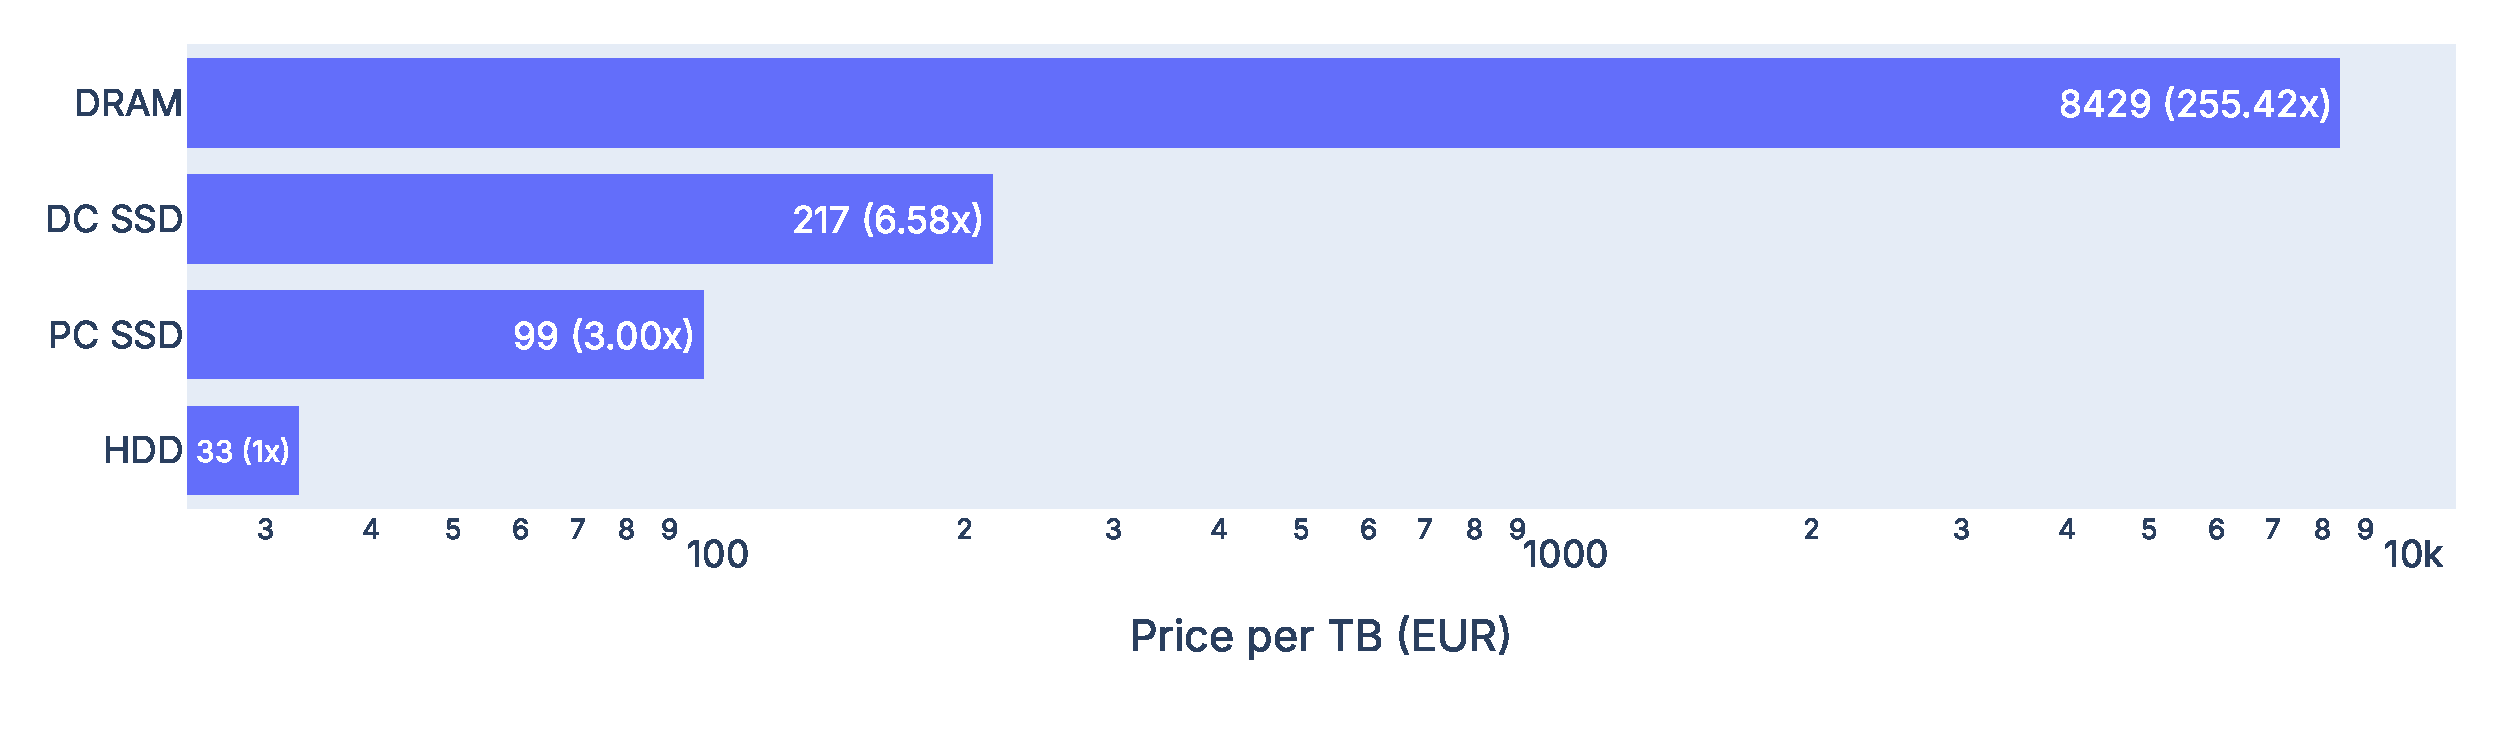
\includegraphics[width=\textwidth]{assets/charts/storage_price.pdf}
    \caption[Data Storage Price Comparison]{
    The normalized price (in Euros per terabyte) of selected storage media as well
    as \ac{DRAM}, as of 12.01.2026 (logarithmic scale) 
     }
    \label{fig:storage-price-comparison}
\end{figure}

In general, mechanical hard drives currently cost less than \acp{SSD} per
gigabyte of storage, while datacenter-grade \acp{SSD} can be significantly more
costly than standard \acp{SSD}. In this case, there is a direct trade-off
between performance and capacity, and not all workloads will necessarily benefit
from improvements to these characteristics. Real-world workloads could vary
significantly in the way that they access the file system---some workloads may
benefit from large, sequential file access, while others could be more random in
nature (see \Cref{sec:access-patterns}). Furthermore, there could be use
cases benefitting purely from capacity over other factors.

Determining which metrics are important for the workloads users will run
can therefore be difficult. However, there exist standardized benchmarks for 
\ac{HPC} storage systems, which aim to cover a wide range of access patterns 
and file sizes, with the goal of providing the best and worst case performance
results for comparison with other systems.

\subsubsection{Benchmarking Tools}
\label{sec:benchmarking-tools}

\ac{IOR} is a storage performance benchmarking tool initially developed at the
\ac{LLNL} in the early 2000s to test the \ac{I/O} performance of the
storage system used in their \ac{HPC}
cluster\footnote{\url{https://web.archive.org/web/20021110104515/https://www.llnl.gov/asci/purple/benchmarks/limited/ior/}.
Archived from the original page, dated 19.09.2001. Accessed 12.01.2026.}. Since
its original implementation, \ac{IOR} remains in active use for the evaluation of
file system performance in \ac{HPC}, with additional features and storage backends
supported\footnote{\url{https://github.com/hpc/ior}. Accessed 24.02.2026.}. Unlike many traditional
benchmarking tools, \ac{IOR} allows for clients running the benchmark to communicate
between each other in order to synchronize their operations and run in parallel.
This feature has the benefit of potentially producing more accurate results, as
well as more closely mimicking the behaviour of \ac{HPC} workloads, which can be
distributed among a large number of nodes. These nodes compete for access to the
same shared storage (e.g., a file system containing datasets for distributed
analysis), which can place a uniquely stressful load on such storage systems.

The mdtest benchmark, included as part of the \ac{IOR} repository, uses the same storage interfaces as the \ac{IOR} benchmarks. However, it is intended to test the metadata performance of \ac{HPC} file systems. Metadata, in this context, refers to the ancillary data stored alongside the contents of the files themselves, such as file names, attributes, folders, and storage locations. To that end, it supports the benchmarking of various operations, such as opening and closing files and directories and stat operations, used for reading attributes such as file size.

IO500\footnote{\url{https://github.com/io500/io500}. Accessed 24.02.2026.} is a standardized storage performance benchmark suite combining the \ac{IOR}
and mdtest benchmarks as well as runs of the find tool, the latter of which is
used to evaluate the performance of file searches. Instead of targeting a
specific use case, it provides a composite score, as well as sub-scores for
different performance profiles, such as ``easy'' \ac{IOR} performance (sequential
reads of a comparatively small number of large files) and ``hard'' mdtest
performance (large numbers of file operations). This establishes a bounding box
for storage performance by providing both worst-case and best-case bandwidth and
metadata results. These results can be compared with the access patterns of
production workloads in order to form a rough prediction of the expected range
in which the workload is expected to perform, given the benchmark results.
Naturally, this raises the question of which access patterns production
\ac{HPC} workloads typically exhibit.

\subsection{\acs{HPC} \acs{I/O} Access Patterns}
\label{sec:access-patterns}

Shan et al.~\cite{hpc-io-prediction} characterize the \ac{I/O} access patterns of traditional \ac{HPC} applications as primarily sequential, although the access sizes may vary by workload. The authors describe two write patterns:

\begin{itemize}
    \item The per-task (N-to-N) pattern, where each process writes its results to its own independent file
    \item The single-shared-file pattern, where each process writes its results to a block within a single shared output file
\end{itemize}

In both of these patterns, the authors observed that individual tasks write their results sequentially to the file system. Their model using the \ac{IOR} benchmark predicted the performance of these workloads well, with a prediction error of under 10\%. We therefore consider \ac{IOR} a valid proxy for the \ac{I/O} access patterns of these traditional \ac{HPC} applications.

However, the \ac{HPC} landscape has shifted significantly since the release of this 2008 report. In particular, the popularity of \ac{AI}, \ac{ML}, and data analytics workloads has increased rapidly. A recent survey by Lewis et al.~\cite{lewis_io_2025} characterizes the access patterns of these modern applications, demonstrating an access pattern considerably different from those of older \ac{HPC} workloads. In particular, \ac{ML} training workflows, particularly those utilizing methods such as \ac{MBGD}, are characterized by frequent random read accesses to relatively small files. These file operations generate heavy metadata accesses, potentially overwhelming the \ac{MDS} services of parallel file systems such as the surveyed Lustre file system, resulting in bottlenecks to training performance~\cite[p.~18]{lewis_io_2025}.

Beyond the primary \ac{HPC} workloads previously discussed, \ac{HPC} file systems can also be used to support ancillary tasks. While workloads such as software compilation, Git operations, and various other operations in users' home or project directories are less bandwidth-intensive than those of the aforementioned primary workloads, they are often dominated by metadata accesses and involve high numbers of file open, close, stat, and create operations on small files. For example, initializing a standard Python virtual environment without the installation of any additional dependencies creates approximately 1700 small files\footnote{Tested on Python 3.11.9}, and cloning a large Git repository such as that of Ceph's latest release branch\footnote{Git clone of \url{https://github.com/ceph/ceph}, \texttt{tentacle} branch. Accessed 26.02.2026.} creates a directory containing several subdirectories with a total of 19,000 small source and metadata files, with each file ranging from a few kilobytes to megabytes in size.

The performance degradation of such workloads for the performance of networked file systems has been documented. Krotkiewski~\cite{Krotkiewski_2017} demonstrated that small-file operations on the BeeGFS parallel file system incur significant performance penalties due to the overhead and latency introduced by metadata operations. To mitigate this issue, the study stored data within disk images formatted with a regular file system (ext4), which resided on the parallel file system and were mounted locally as loopback devices. This results in metadata operations within the loopback device being performed locally, significantly reducing the load on the parallel file system's metadata servers. This approach significantly improved the performance of metadata-intensive tasks, such as searching for files, deleting complex directory trees, and software compilation, reducing their overall time to complete.

\begin{figure}[htbp]
    \centering
    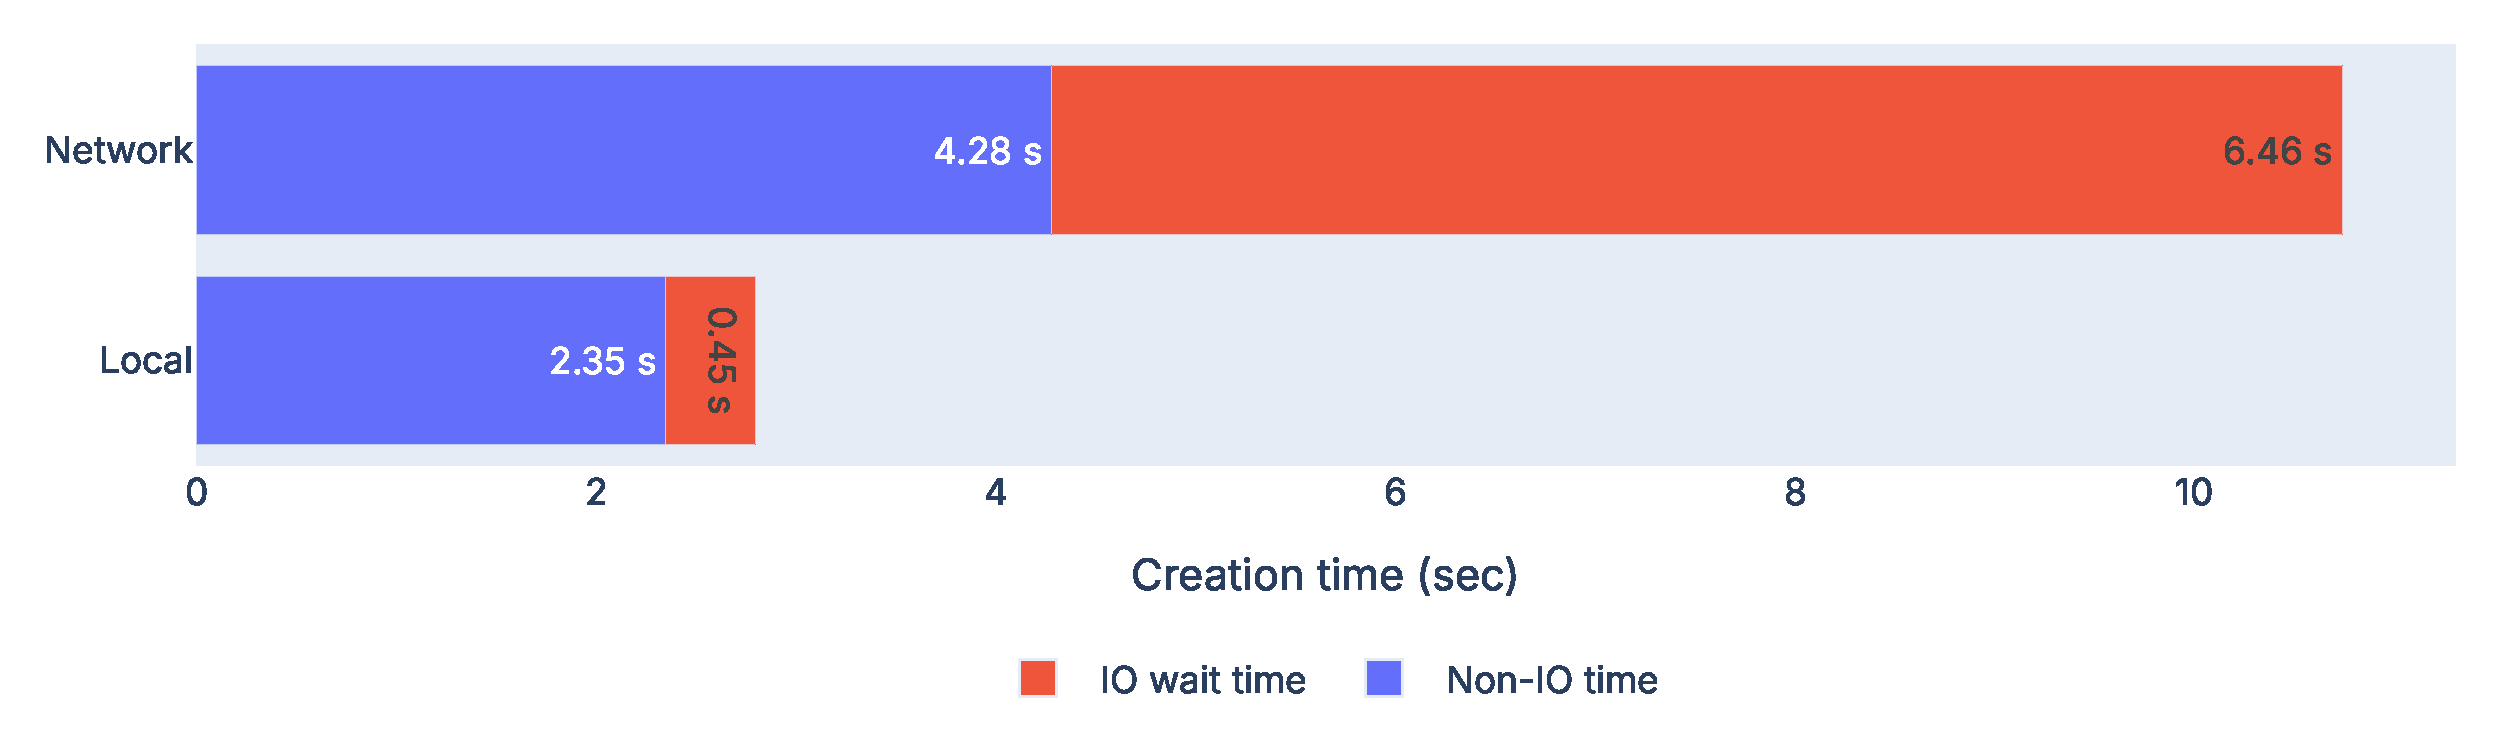
\includegraphics[width=\textwidth]{assets/charts/venv_creation_time.pdf}
    \caption[Python virtual environment creation time]
    {
    Time in seconds required to create a Python virtual environment, with non-\ac{I/O} (user) time and \ac{I/O} wait time shown. When running over a network file system, overall execution time increases significantly, and \ac{I/O} wait time makes up a significant portion of the total time required.
    }
    \label{fig:python-venv-create-time}
\end{figure}

Testing on the production home file system of the \ac{GWDG} \ac{HPC} cluster produces similar results. \Cref{fig:python-venv-create-time} demonstrates the performance impact of the creation of a Python virtual environment on a local tmpfs file system in comparison to a \ac{HPC} file system (in this case, Vast). The creation time of the virtual environment was 3.8$\times$ higher, while the \ac{I/O} wait time increased by over 14$\times$. In total, the 1700 created files had a comparatively small disk utilization of 25 MB, resulting in an effective throughput of 2.35 MB/s, several orders of magnitude lower than the theoretically achievable performance of both the network and storage systems when handling sequential \ac{I/O} operations: for example, creating a 32GB test file using \texttt{dd} resulted in a \acs{CPU}-limited throughput of 1 GB/s, or a throughput roughly 400$\times$ greater than that of the Python virtual environment workload.

As a result, we also consider evaluating Ceph's metadata performance as crucial for determining its viability in \ac{HPC}. This applies not only to modern \ac{AI}/\ac{ML} applications, but also as a general-purpose storage backend for \ac{HPC} home and scratch directories.

\subsection{Ceph Architectural Changes}
\label{sec:ceph-architecture}

The basic architectural concepts within Ceph discussed in \Cref{sec:background} have remained largely stable since the project's inception. However, the implementations of these concepts have evolved significantly over time. One of the most relevant changes are the backends Ceph uses to store data on storage devices~\cite{filesystems-unfit-bluestore}.

Early versions of Ceph relied on the FileStore backend, in which \ac{OSD} data were stored on a traditional file system, generally XFS\footnote{\url{https://docs.ceph.com/en/mimic/man/8/ceph-deploy}. Accessed 24.02.2026.}. While this approach abstracted much of the complexity of storing data on the disk away, it introduced notable performance limitations. In particular, transactional and metadata operations incurred significant overheads. As storage hardware evolved, especially with the growing adoption of fast \ac{NVMe} \acp{SSD}, these limitations became increasingly pronounced, constraining Ceph's scalability and motivating the development of a new storage backend known as BlueStore in 2016. The backend removes the dependency on a traditional file system by communicating with disks directly, as well as integrating journaling directly into the backend itself. This redesign significantly reduced overhead, with initial versions showing substantial improvements of up to 80\% for operations such as object creation~\cite[p.~358]{filesystems-unfit-bluestore}. BlueStore became stable and the default backend in 2017. As of 2023 in the Ceph Reef release, FileStore was removed as a backend entirely\footnote{\url{https://docs.ceph.com/en/reef/ceph-volume/lvm/prepare/\#filestore}. Accessed 24.02.2026.}.

However, advancements in high-performance \ac{NVMe} \acp{SSD} have motivated the development of a new backend known as SeaStore\footnote{\url{https://docs.ceph.com/en/tentacle/dev/seastore/}. Accessed 06.01.2026.}. This implementation is specifically designed to take advantage of high-performance \acp{SSD}. At the time of writing, SeaStore remains an experimental feature under heavy development, and as a result comprehensive performance evaluations are not yet available. Nevertheless, it is likely that future Ceph releases will see SeaStore becoming the standard backend for high-performance \ac{NVMe} \ac{SSD} storage, potentially improving Ceph's performance further.

Therefore, while Ceph is considered a stable and mature platform, it continues to undergo significant changes to its architecture. This history and ongoing development should be considered when reviewing historical performance results for Ceph, especially those using the FileStore backend, as they may no longer be relevant for modern Ceph versions.

\subsection{Ceph Performance}

Although Ceph has existed in some capacity since 2006, uptake in the \ac{HPC} field has been limited. Ceph has seen successful deployments for cloud computing purposes with frameworks such as Rook\footnote{\url{https://rook.io/}. Accessed 26.02.2026.}, as well as for high-reliability data storage in businesses, where the requirements may differ from those of \ac{HPC} workloads. Nevertheless, there have been a few benchmarks of the Ceph file system specifically for \ac{HPC} workloads.

\subsubsection{Early Performance Testing}

One of the earliest performance evaluations of Ceph in an \ac{HPC} context was
performed in 2013 at the \ac{ORNL}~\cite{ceph-ornl-evaluation-filestore}, a
research laboratory which at the time primarily used Lustre for storage of its
data.

The test platform utilized arrays of \ac{SATA} and \ac{SAS} based \acp{HDD} in a \ac{RAID} 6 configuration on top of the FileStore backend.  These benchmarks demonstrated a performance of about 70\% of the raw hardware capabilities. However, due to the design of the FileStore backend---most notably the journaling method---effective write throughput was reduced to half the raw write performance due to the need to initially write data to the journal, followed by backing storage. Despite these limitations, and considering the early state of the Ceph file system at the time, the authors described the tuned performance as satisfactory. 

That being said, the study highlighted one of the largest weaknesses of the Ceph file system at the time, namely journaling overhead of the FileStore backend. The introduction of the BlueStore backend, which substantially altered the way Ceph interacts with disks as described in \Cref{sec:ceph-architecture}, would likely have mitigated some of the issues demonstrated in the paper. However, this paper is still relevant for our analysis as it demonstrates the significant changes and performance improvements Ceph has undergone since its early versions.

\subsubsection{Modern Performance Tests}

More recent evaluations have been performed after Ceph's switch to BlueStore. A study by CERN evaluated Ceph as a data backend for their custom-developed \ac{EOS} system~\cite{cern-evaluating-cephfs-perf}, used for the storage of experiment data (most notably, data gathered as part of particle accelerator experiments). According to the paper, CERN already deploys \ac{CephFS} as \ac{HPC} scratch storage, in addition to other general-purpose use cases. However, limitations such as limited authentication mechanisms and external interfaces---for instance, via HTTP-based access---and the absence of high-throughput testing have limited the application of Ceph to other storage use cases within CERN.

% \cite[p.~2]{cern-evaluating-cephfs-perf}

In the evaluated configuration, \ac{CephFS} was deployed on top of \acs{HDD}-based \acp{OSD} for data storage, with \acp{SSD} being used to store metadata for the \ac{MDS} daemons. Rather than using Ceph's default replica-3 strategy, the system was deployed with erasure coding with a \acs{RAID}-6-like erasure coding configuration from 4 data + 2 coding chunks for 2-disk failure tolerance, to 16 data + 2 coding chunks.

% \cite[pp.~2--3]{cern-evaluating-cephfs-perf}

The results indicate that the per-stream throughput was relatively low with  <400\,MB/s reads and <430\ MB/s writes for a single client. However, aggregate throughput with multiple clients scaled well. Individual nodes were capable of 4.5/5.9 GiB/s of read/write throughput, while the total read/write throughput scaled to 22/34.3 GiB/s~\cite[p.~4]{cern-evaluating-cephfs-perf}. The write performance was deemed to be close to the network limit, while the read performance was likely bottlenecked not by Ceph, but the hard disks themselves.

% \cite[p.~4]{cern-evaluating-cephfs-perf}

Certain issues with Ceph were also reported. A single \ac{OSD} had a disproportionate impact on the overall throughput, dropping write throughput by 80\%. In addition, the default tunable parameters lead to suboptimal performance due to \ac{I/O} stalls at high bandwidths. There was also an issue with \acp{MDS} potentially running out of memory due to the heavy metadata loads \ac{EOS} placed on the file system, however, this was patched in their evaluation and has since been accepted into upstream Ceph\footnote{\url{https://github.com/ceph/ceph/pull/38574}. Accessed 04.01.2026.}.

% \cite[pp.~6--7]{cern-evaluating-cephfs-perf}

While not a peer-reviewed publication, the highest-performing publicly available performance results for Ceph were achieved by Clyso for an unnamed customer in 2023, where they achieved 1\,TiB/s of peak performance for a large-scale Ceph deployment backed by \ac{SSD} storage~\cite{ceph-1tib}. The report details a 63-node cluster consisting of 630 \acp{SSD} in total, with 10 \acp{SSD} and dual 100 Gigabit Ethernet networking per node. The report demonstrated very high aggregate performance with up to 1025/270\,GiB/s of read/write throughput using replication and 547/387\,GiB/s using erasure coding. Additionally, they identified issues with per-node \ac{IOPS} limitations, where each individual node could not exceed 400--600K \ac{IOPS} due to Ceph's messenger implementation, and identified this as a potential source of improvement. However, these performance results were not gathered with \ac{CephFS}, rather with the lower-level \ac{RBD} block storage interface.